In this section we propose a way to model a set of \ewhc{}\new{, $\Lambda$}, as a finite state machine, by utilising the \removed{extended alphabet $\Sigma \left( \strat \right)$}\new{satisfaction set $\sset{}{ \Lambda }$} and the concept of \emph{dominant set}.
The presented approach is invariant to the \removed{actual}control system dynamics. 
For this reason, the resulting model can be used as an interface that separates the software design phase from the stability analysis (Section~\ref{sec:stability}), allowing the complete architecture analysis to be decoupled.

\subsection{Constraint graph}%
\label{sec:constraint_graph}
%
An \ewhc{}, as presented in Definition~\ref{def:new-mk}, can be systematically represented using a \emph{Finite State Machine} (FSM) and the corresponding directed \new{labeled} graph.
\new{%
Each vertex in the graph corresponds to a substring of the last $k$ outcomes of the extended weakly-hard task executions. 
Trivially, there exists no vertices for substrings that do not satisfy the \ewhc{}.
A directed labeled edge connects two vertices if and only if the outcome $\event$ -- the edge's label -- appended to the tail vertex's substring representation would result in an equivalent one to the head vertex's.
This implies that a random walk in the graph corresponds to a random string satisfying the \ewhc{}.
Particularly, this implies that all the walks in the graph corresponds to \emph{all} strings satisfying the \ewhc{}, i.e., $\sset{}{\lambda^{\strat}}$.
}%

\begin{figure}[t]
    \begin{minipage}[c]{0.48\textwidth}
    \begin{center}
        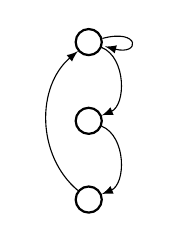
\begin{tikzpicture}[>=latex]
            \node[draw, thick, circle, radius=0.4] (a) at (0,0) {$\cX\cH\cH$};
            \node[draw, thick, circle, radius=0.4] (b) at (0,-1) {$\cH\cH\cM$};
            \node[draw, thick, circle, radius=0.4] (c) at (0,-2) {$\cH\cM\cH$};
            \draw[->] (a) edge [loop right] node[right] {$\cH$} (a);
            \draw[->] (a) edge [bend left=67.5] node[right] {$\cM$} (b);
            \draw[->] (b) edge [bend left=67.5] node[right] {$\cH$} (c);
            \draw[->] (c) edge [bend left=50] node[left] {$\cH$} (a);
        \end{tikzpicture}

        (Example~\ref{ex:auto-kill})\\[1pt]
        $\lambda^{\strat} = \overbar{\binom{1}{3}}^{\text{Kill}}$
    \end{center}
\end{minipage}
%
    \begin{minipage}[c]{0.48\textwidth}
    \begin{center}
        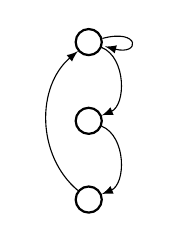
\begin{tikzpicture}[>=latex]
            \node[draw, thick, circle, radius=0.4] (a) at (0,0) {$\cX\cT\cH$};
            \node[draw, thick, circle, radius=0.4] (b) at (0,-1) {$\cT\cH\cM$};
            \node[draw, thick, circle, radius=0.4] (c) at (0,-2) {$\cH\cM\cR$};
            \draw[->] (a) edge [loop right] node[right] {$\cH$} (a);
            \draw[->] (a) edge [bend left=67.5] node[right] {$\cM$} (b);
            \draw[->] (b) edge [bend left=67.5] node[right] {$\cR$} (c);
            \draw[->] (c) edge [bend left=50] node[left] {$\cH$} (a);
        \end{tikzpicture}

        (Example~\ref{ex:auto-skip})\\[1pt]
        $\lambda^{\strat} = \overbar{\binom{1}{3}}^{\text{Skip-Next}}$
    \end{center}
\end{minipage}
%
    \caption{Minimal graph $\GG{\lambda^{\strat}}^*$ for Examples 1 and 2.}
    \label{fig:min-graph}
\end{figure}

We denote the graph corresponding to a task $\tau\vdash\lambda^{\strat}$ \removed{(recall $\lambda \equiv \lambda_{\strat}$)}with the symbol $\GG{\lambda^{\strat}} = (\VV{\lambda^{\strat}}, \EE{\lambda^{\strat}})$.
Here, $\VV{\lambda^{\strat}}$ represents the set of \removed{\emph{nodes}}\new{\emph{vertices}} in the graph and $\EE{\lambda^{\strat}}$ represents the set of \removed{\emph{transitions}}\new{\emph{edges} (also denoted \emph{transitions})}.
Each \removed{node in $\VV{\lambda^{\strat}}$}\new{vertex $v_i \in \VV{\lambda^{\strat}}$} corresponds to a \removed{\emph{word}}\new{string} $\astring_i \in \sset{k}{\lambda^{\strat}}$.
\removed{A \emph{slice} $\astring_i\left(a..b\right)$ of a word is a new word obtained from $\astring_i$ by extracting only the characters starting at position $a$ and ending at position $b$ (both included).}\new{A \emph{substring} $\astring_i\left(a..b\right)$ of $\astring_i = \left\{ \event_1, \dots, \event_N \right\}$ is a new string containing the characters from position $a$ to position $b$, i.e., $\astring_i\left(a..b\right) = \left\{ \event_a, \dots, \event_b \right\}$.}
\removed{%
We assume the initial position in the string to be position $1$.
Furthermore,}We use $\astring_i\left(a..\text{end}\right)$ to indicate the \removed{slice}\new{substring} from position $a$ till the end of \removed{the word}\new{$\astring_i$}.
%
A transition \removed{$c_{i, j} \in \EE{\lambda^{\strat}}$}\new{$e = (v_i,v_j,\event)\in \EE{\lambda^{\strat}}$,} takes us from \removed{node}\new{vertex} $v_i$ to \removed{node}\new{vertex} $v_j$ \removed{.
The transition is labeled by a character $c \in \Sigma\left(\strat\right)$.}\new{and is labeled by the character $\event \in \Sigma\left(\strat\right)$.}
\removed{Node}\new{Vertex} $v_j$ is said to be a direct successor of $v_i$ if concatenating \new{the}character $\event$ to the end of \new{the vertex's string} $\astring_i\left(2..end\right)$ gives $\astring_j$.

Intuitively, a graph $\GG{\lambda^{\strat}}$ has \emph{at most} a number of \removed{nodes}\new{vertices} equal to the cardinality of the set of feasible \removed{words}\new{strings} $\sset{k}{\lambda^{\strat}}$, or formally $\abs{\VV{\lambda^{\strat}}} \leq \abs{\sset{k}{\lambda^{\strat}}}$.
\removed{%
    Building the graph $\GG{\lambda^{\strat}}$ with a number of states $\abs{\VV{\lambda^{\strat}}} = \abs{\sset{k}{\lambda^{\strat}}}$ is always possible, but it would unnecessarily worsen the computational complexity of the problem.

A \emph{minimal state machine realisation} $\GG{\lambda^{\strat}}^*=(\VV{\lambda^{\strat}}^*, \EE{\lambda^{\strat}}^*)$ is easily obtained from $\GG{\lambda^{\strat}}$ using standard techniques~\cite{Hopcroft:2001}.}\new{However, to avoid unnecessary complexity, a \emph{minimal FSM} $\GG{\lambda^{\strat}}^*=(\VV{\lambda^{\strat}}^*, \EE{\lambda^{\strat}}^*)$ is easily obtained from $\GG{\lambda^{\strat}}$ using standard techniques~\cite{Hopcroft:2001}.}
\removed{For each node $w_i$ we observe its successors $\{v_k\}$.}Given two \removed{nodes}\new{vertices} $v_{i}$ and $v_{j}$, if they \removed{have}\new{share} the same successors with the same transition \removed{events}\new{labels (i.e., outcomes)} $\event$ they are considered equivalent and thereby combined.
The differing characters in \new{the string representations of} $v_i$ and $v_j$ are replaced by an \removed{\emph{any character}} \new{\emph{any outcome}} token, which we denote with $\cX$.
This process is repeated until the \removed{state machine}\new{FSM} can no longer be reduced.
%
When considering the Skip-Next strategy, an additional auxiliary token $\cT$ is introduced to represent all \removed{events}\new{outcomes} where a job is completed (ergo; $\cT = \left\{ \cH,\, \cR \right\}$).
\removed{This token is necessary to describe $\GG{\lambda^{\strat}}$, since job completions from $\cH$ and $\cR$ events are equivalent for any arbitrary $\lambda^{\text{Skip-Next}}$ constraint.}


%\afterpage{%
%    \clearpage
    \begin{figure*}[h]
        \begin{minipage}[c]{0.4\textwidth}
    \begin{center}
        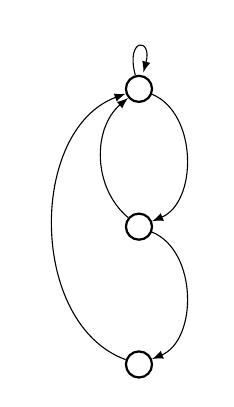
\begin{tikzpicture}[>=latex]
            \node[draw, thick, circle, radius=0.4] (a) at (0,0) {$\textcolor{white}{\cH}\cX\cX\cH\textcolor{white}{\cH}$};
            \node[draw, thick, circle, radius=0.4] (b) at (0,-1.75) {$\textcolor{white}{\cH}\cX\cH\cM\textcolor{white}{\cH}$};
            \node[draw, thick, circle, radius=0.4] (c) at (0,-3.5) {$\textcolor{white}{\cH}\cH\cM\cM\textcolor{white}{\cH}$};
            \draw[->] (a) edge [loop above] node[above] {$\cH$} (a);
            \draw[->] (a) edge [bend left=67.5] node[right] {$\cM$} (b);
            \draw[->] (b) edge [bend left=50] node[left] {$\cH$} (a);
            \draw[->] (b) edge [bend left=67.5] node[right] {$\cM$} (c);
            \draw[->] (c) edge [bend left=70] node[left] {$\cH$} (a);
        \end{tikzpicture}

        (Constraint 1)\\[1pt]
        $\lambda^{\strat}_1 = \overbar{\left<2\right>}^{\text{Kill}}$
    \end{center}
\end{minipage}
\hspace{1cm}
\begin{minipage}[c]{\textwidth}
    \begin{center}
        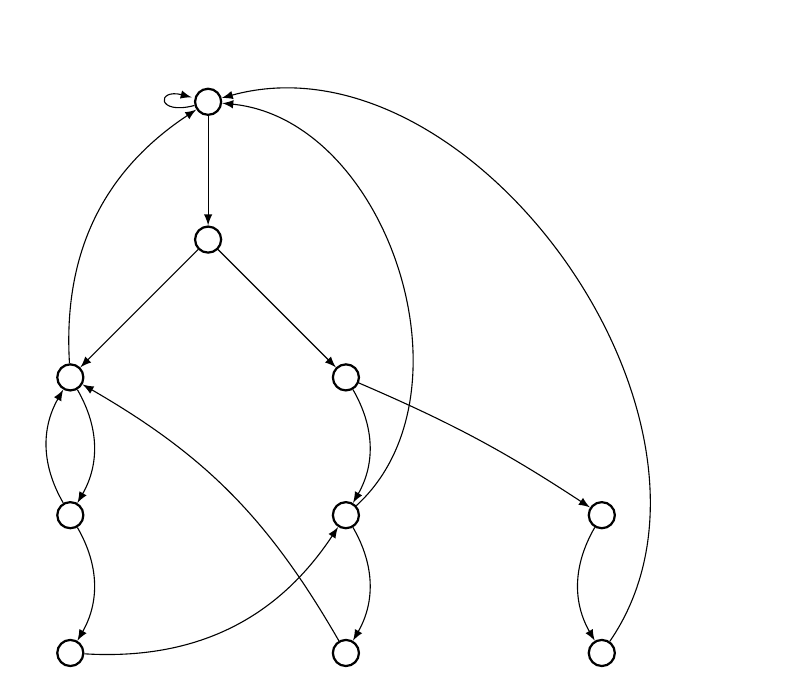
\begin{tikzpicture}[>=latex]
            \node[draw, thick, circle, radius=0.4] (a) at (0,0) {$\cX\cX\cX\cH\cH$};
            \node[draw, thick, circle, radius=0.4] (b) at (0,-1.75) {$\cX\cX\cH\cH\cM$};
            \node[draw, thick, circle, radius=0.4] (c) at (-1.75,-3.5) {$\cX\cX\cH\cM\cH$};
            \node[draw, thick, circle, radius=0.4] (d) at (-1.75,-5.25) {$\cX\cH\cM\cH\cM$};
            \node[draw, thick, circle, radius=0.4] (e) at (-1.75,-7) {$\cH\cM\cH\cM\cM$};
            \node[draw, thick, circle, radius=0.4] (f) at (1.75,-3.5) {$\cX\cH\cH\cM\cM$};
            \node[draw, thick, circle, radius=0.4] (g) at (1.75,-5.25) {$\cX\cH\cM\cM\cH$};
            \node[draw, thick, circle, radius=0.4] (h) at (1.75,-7) {$\cH\cM\cM\cH\cM$};
            \node[draw, thick, circle, radius=0.4] (i) at (5,-5.25) {$\cH\cH\cM\cM\cM$};
            \node[draw, thick, circle, radius=0.4] (j) at (5,-7) {$\cH\cM\cM\cM\cH$};

            \draw[->] (a) edge [loop left] node[left] {$\cH$} (a);
            \draw[->] (a) edge [] node[right] {$\cM$} (b);
            \draw[->] (b) edge node [above] {$\cH$} (c);
            \draw[->] (b) edge node [above] {$\cM$} (f);
            \draw[->] (c) edge [bend left] node [left] {$\cH$} (a);
            \draw[->] (c) edge [bend left] node [right] {$\cM$} (d);
            \draw[->] (d) edge [bend left] node [left] {$\cH$} (c);
            \draw[->] (d) edge [bend left] node [right] {$\cM$} (e);
            \draw[->] (e) edge [bend right] node [below] {$\cH$} (g);
            \draw[->] (f) edge [bend left] node [right] {$\cH$} (g);
            \draw[->] (f) edge [bend left=5] node [above] {$\cM$} (i);
            \draw[->] (g) edge [bend right = 66] node [right] {$\cH$} (a);
            \draw[->] (g) edge [bend left] node [right] {$\cM$} (h);
            \draw[->] (h) edge [bend right = 15] node [above] {$\cH$} (c);
            \draw[->] (i) edge [bend right] node [left] {$\cH$} (j);
            \draw[->] (j) edge [bend right = 70] node [right] {$\cH$} (a);

        \end{tikzpicture}

        (Constraint 2)\\[1pt]
        $\lambda^{\strat}_2 = \overbar{\binom{3}{5}}^{\text{Kill}}$
    \end{center}
\end{minipage}
\hspace{1cm}
\begin{minipage}[c]{0.8\textwidth}
    \begin{center}
        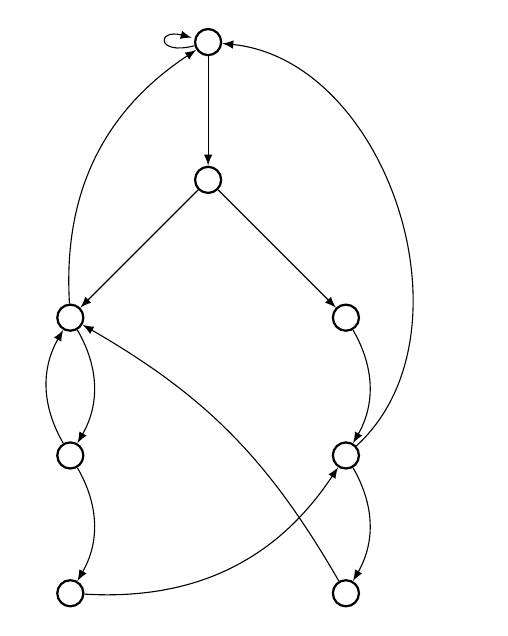
\begin{tikzpicture}[>=latex]
            \node[draw, thick, circle, radius=0.4] (a) at (0,0) {$\cX\cX\cX\cH\cH$};
            \node[draw, thick, circle, radius=0.4] (b) at (0,-1.75) {$\cX\cX\cH\cH\cM$};
            \node[draw, thick, circle, radius=0.4] (c) at (-1.75,-3.5) {$\cX\cX\cH\cM\cH$};
            \node[draw, thick, circle, radius=0.4] (d) at (-1.75,-5.25) {$\cX\cH\cM\cH\cM$};
            \node[draw, thick, circle, radius=0.4] (e) at (-1.75,-7) {$\cH\cM\cH\cM\cM$};
            \node[draw, thick, circle, radius=0.4] (f) at (1.75,-3.5) {$\cX\cH\cH\cM\cM$};
            \node[draw, thick, circle, radius=0.4] (g) at (1.75,-5.25) {$\cX\cH\cM\cM\cH$};
            \node[draw, thick, circle, radius=0.4] (h) at (1.75,-7) {$\cH\cM\cM\cH\cM$};

            \draw[->] (a) edge [loop left] node[left] {$\cH$} (a);
            \draw[->] (a) edge [] node[right] {$\cM$} (b);
            \draw[->] (b) edge node [above] {$\cH$} (c);
            \draw[->] (b) edge node [above] {$\cM$} (f);
            \draw[->] (c) edge [bend left] node [left] {$\cH$} (a);
            \draw[->] (c) edge [bend left] node [right] {$\cM$} (d);
            \draw[->] (d) edge [bend left] node [left] {$\cH$} (c);
            \draw[->] (d) edge [bend left] node [right] {$\cM$} (e);
            \draw[->] (e) edge [bend right] node [below] {$\cH$} (g);
            \draw[->] (f) edge [bend left] node [right] {$\cH$} (g);
            \draw[->] (g) edge [bend right = 66] node [right] {$\cH$} (a);
            \draw[->] (g) edge [bend left] node [right] {$\cM$} (h);
            \draw[->] (h) edge [bend right = 15] node [above] {$\cH$} (c);

        \end{tikzpicture}

        (Result)\\[1pt]
        $\Lambda^{\strat}_0 = \left\{ \lambda^{\strat}_1,\, \lambda^{\strat}_2 \right\}$
    \end{center}
\end{minipage}

        \caption{Minimal graphs $\GG{\lambda^{\strat}_1}^*$, $\GG{\lambda^{\strat}_2}^*$, and $\GG{\Lambda^{\strat}_0}^*$ for Example~\ref{ex:auto-comb}.}
        \label{fig:multi-graphs}
    \end{figure*}
%    \clearpage
%}

\begin{example}%
    \label{ex:auto-kill}%
    \emph{Given an \ewhc{},} $\lambda^{\strat} = \overbar{\binom{1}{3}}^{\text{Kill}}$\emph{, the minimal realisation $\GG{\lambda^{\strat}}^*$ is shown in the left-hand side of Figure~\ref{fig:min-graph}.
    The \removed{node}\new{vertex represented by the string} $\cX\cH\cH$ is obtained by merging $\cH\cH\cH$ and $\cM\cH\cH$.
    \removed{It can be interpreted as the first character not affecting the possible transitions.}}
\end{example}

\begin{example}%
    \label{ex:auto-skip}%
    \emph{Given an \ewhc{},} $\lambda^{\strat} = \overbar{\binom{1}{3}}^{\text{Skip-Next}}$\emph{, the minimal realisation $\GG{\lambda^{\strat}}^*$ is shown in the right-hand side of Figure~\ref{fig:min-graph}.}
\end{example}

\removed{The similarities between Kill and Skip-Next under the extended notation become apparent as soon as we compare the minimal state machines in Figure~\ref{fig:min-graph}.
The resulting graphs}\new{The minimal FSM for Kill and Skip-Next in Figure~\ref{fig:min-graph}} have identical number of \removed{nodes}\new{vertices} but slightly different \removed{events}\new{transitions}.
\new{%
This is not a coincidence, but follows directly from Definition~\ref{def:new-mk} and the extended alphabet $\Sigma\left(\strat\right)$.
A hit ($\cH$) and a recovery ($\cR$) are both considered job completions, which is why the graphs for the Kill and Skip-Next strategies have the same structure.
It is only the first job completion after a period of no job completions ($\cM$) that differ.}%
However, \removed{this difference becomes significant when analysing}\new{the different transitions of the two graphs affect} the corresponding closed-loop systems, as will be clear in Section~\ref{sec:stability}.

\subsection{Dealing with multiple constraints}
\label{sec:mult-const}

The approach presented above for constructing a minimal FSM can be extended to the case where the task $\tau$ is subject to a set of multiple \ewhc{}\removed{, in any combination of the forms presented in Definition~\ref{def:new-mk}}. 
Such a set is formally denoted as $\Lambda^{\strat}$.\removed{, but again to simplify the notation, for the remainder of the paper $\Lambda \equiv \Lambda^{\strat}$, unless explicitly stated otherwise.}
%
In order to optimise the problem of building the minimal FSM of the corresponding system, it is beneficial that the set $\Lambda^{\strat}$ contains only constraints that cannot be further reduced using the hardness relations of Definition~\ref{def:domination}. 
\removed{For this reason,}\new{To this end,} we first introduce the new concept of \removed{\emph{dominant constraint set}(or simply dominant set).}\new{\emph{dominant (constraint) set}.}
%
\begin{definition}[Dominant set]%
    \label{def:dominant-set}%
    \removed{Given a set of constraints $\Lambda$ under strategy $\strat$, the set $\Lambda^\star \subseteq \Lambda$ is called the \emph{dominant set} of $\Lambda$ if:}%
    \new{Given a set of \ewhc{}, $\Lambda^{\strat}$, the set $\Lambda^{\strat}_0 \subseteq \Lambda^{\strat}$ is called the \emph{dominant set} of $\Lambda^{\strat}$ if:}
    \begin{enumerate}[label=(\roman*)]
        \item $\lambda^{\strat}_i,\lambda^{\strat}_j \in \Lambda^{\strat}_0 \,\,\implies \lambda^{\strat}_i \npreceq \lambda^{\strat}_j,\, \forall i \neq j,$
        \item $\lambda^{\strat}_i \in \Lambda^{\strat} \setminus \Lambda^{\strat}_0 \implies
            \lambda^{\strat}_j \preceq \lambda^{\strat}_i,\, \exists \lambda^{\strat}_j \in \Lambda^{\strat}_0.$
    \end{enumerate}
\end{definition}

Building upon Definition~\ref{def:satisfaction}, the satisfaction set of $\Lambda^{\strat}_0$ can be derived as follows, for $N\geq 1$:
%
\begin{equation}
    \label{eq:satisfaction-multi}
    \sset{N}{\Lambda^{\strat}_0} \equiv \bigcap_{\lambda^{\strat}_i \in \Lambda^{\strat}_0} \sset{N}{\lambda^{\strat}_i}.
\end{equation}
%
We can then obtain a minimal graph \removed{$\GG{\Lambda^{\strat}_0}^*=(\VV{\Lambda^{\strat}_0}^*, \EE{\Lambda^{\strat}_0}^*)$}\new{$\GG{\Lambda^{\strat}_0}^*$} following a procedure similar to the one presented for a single constraint $\lambda^{\strat}$ in Section~\ref{sec:state-machine}.
As a first step, the length of the \removed{words}\new{strings} in each \removed{node}\new{vertex} of the corresponding graph must be defined.
Since $\Lambda^{\strat}_0$ may contain constraints with different window values, the choice is not straightforward.
We propose a safe assumption about the \removed{words}\new{string} length $k_0$, defined as $\,k_0 = \max_{k} \lambda^{\strat},\,\, \forall \lambda^{\strat} \in \Lambda^{\strat}_0$\removed{ (recall that each \ewhc{} is window dependent)}.
An algorithm can then be built that \removed{, recursively,}adds \removed{nodes $\alpha_i \in \sset{k_0}{ \Lambda^{\strat}_0 }$}\new{vertices, with string representations $\astring_i \in \sset{k_0}{ \Lambda^{\strat}_0 }$,} to the graph until a minimal realisation is generated.
The obtained graph is finally passed through a post-processing step (strategy-dependent) that assigns \new{the} appropriate transitions \removed{$c_{i, j}$}in order to obtain a correct minimal FSM realisation $\GG{\Lambda^{\strat}_0}^*$.

\begin{example}%
    \label{ex:auto-comb}%
    \emph{Given two \ewhc{},} $\lambda^{\strat}_1 = \overbar{\left<2\right>}^{\text{Kill}}$\emph{ and } $\lambda^{\strat}_2 = \overbar{\binom{3}{5}}^{\text{Kill}}$\emph{, the minimal realisation graphs $\GG{\lambda^{\strat}_1}^*$ and $\GG{\lambda^{\strat}_2}^*$ are shown as the leftmost and middle graphs of Figure~\ref{fig:multi-graphs}.
    Generating the graph $\GG{\Lambda^{\strat}_0}^*$ from the dominant set $\Lambda^{\strat}_0 = \{ \lambda^{\strat}_1, \lambda^{\strat}_2 \}$ results in the rightmost graph of Figure~\ref{fig:multi-graphs}, satisfying both $\lambda^{\strat}_1$ and $\lambda^{\strat}_2$.}
    \removed{\emph{A similar result can be obtained for the} Skip-Next \emph{strategy\removed{, by using its corresponding alphabet.}}}
\end{example}


Building a minimal FSM by choosing the dominant set $\Lambda^{\strat}_0$ \removed{is useful to improve}\new{improves} the computational performance of the analysis \removed{algorithms}.
Nonetheless, the analysis presented in the following sections can be applied to any graph built from a given set $\Lambda^{\strat}$.
To limit complexity in the notation, and for the sake of generality, all future steps will \removed{be defined using}\new{consider} a generic graph \removed{$\GG{\Lambda^{\strat}}$}\new{$\GG{\Lambda^{\strat}}=(\VV{\Lambda^{\strat}}, \EE{\Lambda^{\strat}})$}.


\subsection{Dynamic model of a graph}
\label{ssec:dynamicgraph}

\removed{An arbitrary walk of $N$ steps in the state machine $\GG{\Lambda}$ corresponds to a distinct sequence $\alpha \in \sset{N}{ \Lambda }$.}
Extracting all the transitions \removed{$c_{i, j} \in \EE{\Lambda}$}\new{in $\EE{\Lambda^\strat}$} corresponding to a \removed{particular event}\new{character} $\event$ yields what is generally known as a \emph{directed adjacency matrix}~\cite{xu2012matrix}, denoted here as a \emph{transition matrix}. \removed{due to its connection to the transition event $\event$.}
\begin{definition}[Transition matrix]
    \label{def:transition}
    Given a graph $\GG{\Lambda^\strat}$, the \removed{directed adjacency matrix (or \emph{transition matrix}),}\new{\emph{transition matrix}} $F_{\event} ( \GG{\Lambda^\strat} ) \in \R^{\abs{\VV{\Lambda^\strat}} \times \abs{\VV{\Lambda^\strat}}}$ with $\event\in\Sigma\left(\strat\right)$, is computed as $F_{\event} ( \GG{\Lambda^\strat} ) = \{f_{i,j}(\event)\}$ with
    \removed{
    \begin{equation*}
        f_{i,j}\funof{c}=
        \begin{cases}
            1, &\text{ if } c_{j,i} \in \EE{\Lambda} \\
            0, &\text{ otherwise}
        \end{cases}
    \end{equation*}  
    }%      
    %
    \begin{equation*}
        f_{i,j}\funof{\event}=
        \begin{cases}
            1, &\text{ if } \exists \, e=(v_j,v_i,\event) \in \EE{\Lambda^\strat} \\
            0, &\text{ otherwise.}
        \end{cases}
        \end{equation*}%
\end{definition}
%
\removed{The walk (i.e., the completion sequence) can then be expressed in terms of a left-multiplication between the corresponding transition matrices.}%
Since there can only exist \emph{at most one} successor from each node with \removed{the}\new{a} transition \removed{event}\new{labeled with} $\event$, the transition matrix $F_\event$ will thus have a column sum of either 1 or 0.
\removed{Finally,}We introduce a vector $q_t\in \R^{\abs{\VV{\Lambda^\strat}}}$ called \emph{G-state} (for graph state), representing the state of the given graph $\GG{\Lambda^\strat}$, which is associated to the interval $\pi_t$.
This vector is formally defined as follows.
\begin{definition}[G-state $q_t$]\label{def:qt}
    Given a graph $\GG{\Lambda^\strat} = (\VV{\Lambda^\strat}, \EE{\Lambda^\strat})$ and a sequence $\astring \in \Sigma\left( \strat \right)^N$, for $k = \abs{v},\,\, v\in\VV{\Lambda^\strat}$, we define $q_t\in \R^{\abs{\VV{\Lambda}}}$, where the $i$-th element \removed{$q_t(i)$}\new{$q_{t,i}$} is defined as:
    \begin{equation*}
        q_{t,i}=
        \begin{cases}
            1, &\text{ if } \astring\left(t-k..t-1\right) \equiv v_i \in \VV{\Lambda^\strat} \\
            0, &\text{otherwise}.
        \end{cases}
    \end{equation*}
\end{definition}
In other words, the G-state $q_t$ is the vector representation of the \removed{index corresponding to the node}\new{vertex} we are \emph{leaving} at step $t$.
\removed{Particularly, for all feasible sequences $\alpha \in \sset{N}{ \Lambda }$, $q_t$ contains \emph{exactly} one $1$ at index $i$, where $w_i \equiv \alpha(t-k..t-1) \in \VV{\Lambda}$ (all other values are $0$).
However, for an arbitrary sequence $\alpha \in \Sigma \left( \strat \right)^N$, the G-state contains \emph{at most} one $1$.}In this definition, $q_t=0$ means that the transition \removed{$\alpha_{t-1}$}\new{at step $t-1$} was infeasible for the graph. The G-state dynamics, given an arbitrary sequence \removed{$\alpha$}\new{$\astring=\{\alpha_1,\dots,\alpha_t,\dots,\}$}, \removed{can then easily be defined as $q_{t+1} = F_\event^{\strat}\cdot q_t$, with $\event=\alpha_t$}\new{is then defined as $q_{t+1} = F_{\event} ( \GG{\Lambda^\strat} )\cdot q_t$}.
\removed{Trivially}\new{Hence,} the following property from~\cite{xu2012matrix} holds.
\begin{lemma}[\removed{Transition matrix of an}Infeasible sequence]
    \label{cor:Fseqnotinlambda}
    If $\astring \notin \sset{N}{ \Lambda^\strat }$, then $F_{\astring} ( \GG{\Lambda^\strat} ) =
    F_{\event_N} ( \GG{\Lambda^\strat} )\cdots F_{\event_2} ( \GG{\Lambda^\strat} )\cdot F_{\event_1} ( \GG{\Lambda^\strat} ) = 0$
\end{lemma}
Thus, if $q_t=0$ for any $t$, then $q_{t'}=0$ for $t' \geq t$.
